\documentclass[11pt,a4paper]{article}
\usepackage[T1]{fontenc}
\usepackage[utf8]{inputenc}
\usepackage{lmodern}
\usepackage{textcomp}
\usepackage[left=1.8cm,right=1.8cm,top=2.3cm,bottom=2.2cm,headheight=14pt,headsep=8pt]{geometry}
\usepackage{multicol}
\usepackage{xcolor}
\usepackage{fancyhdr}
\usepackage{graphicx}
\usepackage{array}
\usepackage{amsmath,amssymb}
\usepackage{setspace}
\usepackage{longtable}
\graphicspath{{../}}
\definecolor{ygreen}{RGB}{46,139,87}
\renewcommand{\normalsize}{\fontsize{10.9}{13.4}\selectfont}
\renewcommand{\familydefault}{\rmdefault}
\setlength{\parindent}{0pt}
\setlength{\columnsep}{0.8cm}
\setlength{\columnseprule}{0.4pt}
\setlength{\multicolsep}{3pt plus 1pt minus 1pt}
\renewcommand{\textsubscript}[1]{\ensuremath{_{\text{\fontsize{8}{8}\selectfont #1}}}}
\renewcommand{\textsuperscript}[1]{\ensuremath{^{\text{\fontsize{8}{8}\selectfont #1}}}}
\newcommand{\diqqat}[1]{\par\smallskip\noindent\textbf{Diqqat!} #1\par\medskip}
\newcommand{\javob}{\par\smallskip\noindent\textbf{Javob:} \rule[-2pt]{7.5cm}{0.4pt}\par\smallskip\noindent\textbf{Diqqat!} Javobingizni javoblar varaqasiga ko`chirib yozing.\par\medskip}
\pagestyle{fancy}
\fancyhf{}
\renewcommand{\headrulewidth}{0.4pt}
\fancyhead[L]{\textit{Milliy sertifikat 2026. Kimyo}}
\fancyhead[R]{9-variant}
\fancyfoot[L]{\fontsize{8}{9}\selectfont \textcopyright{} Colba maktabi, 2026}
\fancyfoot[C]{\thepage}
\fancypagestyle{first}{\fancyhf{}\renewcommand{\headrulewidth}{0pt}\fancyfoot[L]{\fontsize{8}{9}\selectfont \textcopyright{} Colba maktabi, 2026}\fancyfoot[C]{\thepage}}
\begin{document}
\normalsize
\thispagestyle{first}
\noindent\fcolorbox{ygreen}{white}{\parbox{\dimexpr\linewidth-2\fboxsep-2\fboxrule\relax}{%
\textbf{\fontsize{13}{15}\selectfont Nazorat testi}\ \textit{\fontsize{10}{12}\selectfont $\cdot$ Aralash test $\cdot$ 9-variant}\hfill
\begin{tabular}[t]{@{}r@{}}\textit{Milliy sertifikat 2026. Kimyo}\\ \textbf{\textit{\fontsize{8}{9}\selectfont Vaqt:}} \textit{\fontsize{10}{12}\selectfont 180 daqiqa}\end{tabular}}}
\par\medskip
\noindent\textit{Davriy jadvaldan foydalanish mumkin.}
\par\medskip
\begin{multicols}{2}
\noindent\textbf{1.} Kislotada Fe bo`lagi eritilganda ajralgan vodorod hajmining vaqtga bog`liqligi grafikda berilgan.
\begin{center}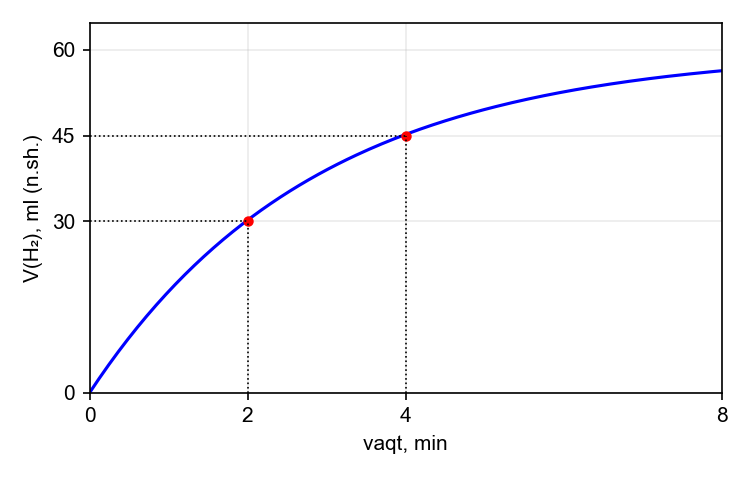
\includegraphics[width=0.86\linewidth]{rasmlar/gen/gv_v09_0.png}\end{center}
2-minutdan 4-minutgacha vodorod ajralishining o`rtacha \textbf{tezligini (ml/min) hisoblang.}

\noindent A)~\textsl{7,5} \hfill B)~\textsl{15} \hfill C)~\textsl{22,5} \hfill D)~\textsl{3,75}\par
\vspace{4pt}
\noindent\textbf{2.} Quyidagi zarrachalardan qaysilari neon atomi bilan izoelektron? 1) Al\textsuperscript{3+}; 2) Cl\textsuperscript{$-$}; 3) S\textsuperscript{2$-$}; 4) F\textsuperscript{$-$}

\noindent A)~\textsl{2, 3, 4} \hfill B)~\textsl{1, 4} \hfill C)~\textsl{1, 2} \hfill D)~\textsl{2, 4}\par
\vspace{4pt}
\end{multicols}
\noindent\textbf{3.} NH\textsubscript{4}Cl tuzining eruvchanligi (g/100 g suv) haroratga bog`liq jadvalda keltirilgan:
\begin{center}
\renewcommand{\arraystretch}{1.15}
\begin{tabular}{|c|c|c|c|c|}\hline
\textbf{t, \textdegree{}C} & \textbf{0} & \textbf{20} & \textbf{40} & \textbf{60} \\ \hline
S, g/100 g suv & 13 & 32 & 64 & 110 \\ \hline
\end{tabular}
\end{center}
40 \textdegree{}C da tayyorlangan to`yingan 410 g eritma 20 \textdegree{}C gacha sovitildi. Cho`kmaga tushgan tuz \textbf{massasini (g) aniqlang.}

\noindent A)~\textsl{160} \hfill B)~\textsl{80} \hfill C)~\textsl{40} \hfill D)~\textsl{120}\par
\vspace{4pt}
\begin{multicols}{2}
\noindent\textbf{4.} Quyidagi tuzlarning qaysilari suvli eritmasi ishqoriy muhitga ega? 1) K\textsubscript{3}PO\textsubscript{4}; 2) ZnCl\textsubscript{2}; 3) K\textsubscript{2}SO\textsubscript{4}; 4) NH\textsubscript{4}Cl

\noindent A)~\textsl{2, 3} \hfill B)~\textsl{3} \hfill C)~\textsl{3, 4} \hfill D)~\textsl{1}\par
\vspace{4pt}
\noindent\textbf{5.} \textit{X} moddaning parchalanish reaksiyasida konsentratsiyaning vaqt bo`yicha o`zgarishi jadvalda berilgan:
\begin{center}
\renewcommand{\arraystretch}{1.15}
\begin{tabular}{|c|c|}\hline
\textbf{t, min} & \textbf{c, mol/l} \\ \hline
0 & 1,2 \\ \hline
2 & 1,08 \\ \hline
4 & 0,96 \\ \hline
6 & 0,84 \\ \hline
\end{tabular}
\end{center}
0-minutdan 4-minutgacha o`rtacha tezlikni mol/(l$\cdot$min) \textbf{hisoblang.}

\noindent A)~\textsl{0,06} \hfill B)~\textsl{0,12} \hfill C)~\textsl{0,03} \hfill D)~\textsl{0,24}\par
\vspace{4pt}
\noindent\textbf{6.} Rasmda kristall panjara tuzilishi tasvirlangan.
\begin{center}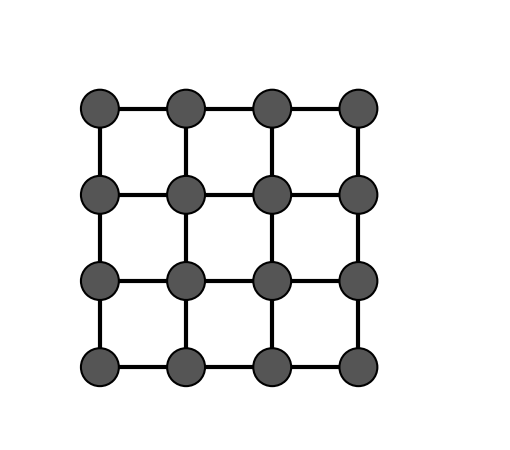
\includegraphics[width=0.86\linewidth]{rasmlar/gen/la_950269.png}\end{center}
Bu panjara qaysi turga kiradi?
\noindent A)~\textsl{ion kristall panjara}\par
\noindent B)~\textsl{atom kristall panjara}\par
\noindent C)~\textsl{molekulyar kristall panjara}\par
\noindent D)~\textsl{metall kristall panjara}\par
\vspace{4pt}
\noindent\textbf{7.} 0,5 M Al\textsubscript{2}(SO\textsubscript{4})\textsubscript{3} eritmasining normal \textbf{konsentratsiyasini (n) aniqlang.}

\noindent A)~\textsl{0,5} \hfill B)~\textsl{3} \hfill C)~\textsl{6} \hfill D)~\textsl{0,083}\par
\vspace{4pt}
\noindent\textbf{8.} NaCl eritmasi inert elektrodlar yordamida 2 A tok kuchi bilan 9650 s elektroliz qilindi. Anodda ajralgan Cl\textsubscript{2} hajmi (l, n.sh.) \textbf{ni toping.}

\noindent A)~\textsl{4,48} \hfill B)~\textsl{1,12} \hfill C)~\textsl{2,24} \hfill D)~\textsl{0,448}\par
\vspace{4pt}
\noindent\textbf{9.} N\textsubscript{2} + 3H\textsubscript{2} $\rightleftarrows$ 2NH\textsubscript{3} reaksiyada muvozanat qaror topganda [N\textsubscript{2}] = 1, [H\textsubscript{2}] = 2, [NH\textsubscript{3}] = 1 mol/l bo`ldi. H\textsubscript{2} ning boshlang`ich \textbf{konsentratsiyasini (mol/l) aniqlang.}

\noindent A)~\textsl{2} \hfill B)~\textsl{4} \hfill C)~\textsl{3} \hfill D)~\textsl{3,5}\par
\vspace{4pt}
\noindent\textbf{10.} Faqat oksidlovchi bo`la oladigan \textbf{ionlarni aniqlang}: 1) Cl\textsuperscript{$-$}; 2) Na\textsuperscript{+}; 3) I\textsuperscript{$-$}; 4) Al\textsuperscript{3+}

\noindent A)~\textsl{3} \hfill B)~\textsl{1, 3} \hfill C)~\textsl{2, 4} \hfill D)~\textsl{1, 4}\par
\vspace{4pt}
\noindent\textbf{11.} ZnSO\textsubscript{4} ning suvli eritmasi inert elektrodlar bilan elektroliz qilinganda qaysi moddalar ajraladi?

\noindent\begin{tabular}{@{}p{0.47\linewidth}@{}p{0.47\linewidth}@{}}
A)~\textsl{Zn, H\textsubscript{2} va O\textsubscript{2}} & B)~\textsl{Cu va Cl\textsubscript{2}} \\
C)~\textsl{H\textsubscript{2} va O\textsubscript{2}} & D)~\textsl{Ag va O\textsubscript{2}} \\
\end{tabular}\par
\vspace{4pt}
\noindent\textbf{12.} 2,5 mol C\textsubscript{2}H\textsubscript{6} tarkibida necha mol atom bor?

\noindent A)~\textsl{17,5} \hfill B)~\textsl{22,5} \hfill C)~\textsl{2,5} \hfill D)~\textsl{20}\par
\vspace{4pt}
\noindent\textbf{13.} 11,7 g NaCl 200 g suvda eritildi. Eritmaning molyal \textbf{konsentratsiyasini (mol/kg) aniqlang.}

\noindent A)~\textsl{0,94} \hfill B)~\textsl{0} \hfill C)~\textsl{1} \hfill D)~\textsl{2}\par
\vspace{4pt}
\noindent\textbf{14.} Reaksiya tenglamasi: ZnO + 2HCl $\to$ ZnCl\textsubscript{2} + H\textsubscript{2}O. Reaksiyaga tarkibida 20\% aralashma bo`lgan 20,25 g namuna (asosiy modda ZnO) kirishdi. HCl \textbf{hajmini (l, n.sh.) hisoblang.}

\noindent A)~\textsl{2,24} \hfill B)~\textsl{17,92} \hfill C)~\textsl{8,96} \hfill D)~\textsl{4,48}\par
\vspace{4pt}
\noindent\textbf{15.} Mg(HCO\textsubscript{3})\textsubscript{2} $\to$ MgCO\textsubscript{3} + CO\textsubscript{2} + H\textsubscript{2}O reaksiyasida 146 g Mg(HCO\textsubscript{3})\textsubscript{2} ishtirok etdi. MgCO\textsubscript{3} \textbf{massasini (g) toping.}

\noindent A)~\textsl{168} \hfill B)~\textsl{42} \hfill C)~\textsl{126} \hfill D)~\textsl{84}\par
\vspace{4pt}
\noindent\textbf{16.} Reaksiya tenglamasi: N\textsubscript{2}O\textsubscript{5} + H\textsubscript{2}O $\to$ 2HNO\textsubscript{3}. Reaksiyaga tarkibida 10\% aralashma bo`lgan 12 g namuna (asosiy modda N\textsubscript{2}O\textsubscript{5}) kirishdi. HNO\textsubscript{3} \textbf{massasini (g) hisoblang.}

\noindent A)~\textsl{12,6} \hfill B)~\textsl{3,15} \hfill C)~\textsl{25,2} \hfill D)~\textsl{6,3}\par
\vspace{4pt}
\noindent\textbf{17.} P $\to$ ? $\to$ ? $\to$ ? o`zgarishlar zanjirida (reagentlar: O\textsubscript{2}, H\textsubscript{2}O, KOH) 3-bosqichda hosil bo`ladigan modda \textbf{formulasini toping.}

\noindent A)~\textsl{K\textsubscript{3}PO\textsubscript{4}} \hfill B)~\textsl{SO\textsubscript{2}} \hfill C)~\textsl{Na\textsubscript{2}O} \hfill D)~\textsl{NaOH}\par
\vspace{4pt}
\noindent\textbf{18.} NH\textsubscript{3} + H\textsubscript{3}PO\textsubscript{4} $\to$ NH\textsubscript{4}H\textsubscript{2}PO\textsubscript{4} jarayoni uchun 98 g H\textsubscript{3}PO\textsubscript{4} olingan (unum 60\%). NH\textsubscript{4}H\textsubscript{2}PO\textsubscript{4} \textbf{massasini (g) aniqlang.}

\noindent A)~\textsl{115} \hfill B)~\textsl{138} \hfill C)~\textsl{69} \hfill D)~\textsl{34,5}\par
\vspace{4pt}
\noindent\textbf{19.} NH\textsubscript{4}NO\textsubscript{3} qizdirilganda qanday moddalar hosil bo`ladi?

\noindent\begin{tabular}{@{}p{0.47\linewidth}@{}p{0.47\linewidth}@{}}
A)~\textsl{Ag, NO\textsubscript{2} va O\textsubscript{2}} & B)~\textsl{N\textsubscript{2}O va H\textsubscript{2}O} \\
C)~\textsl{KNO\textsubscript{2} va O\textsubscript{2}} & D)~\textsl{CuO, NO\textsubscript{2} va O\textsubscript{2}} \\
\end{tabular}\par
\vspace{4pt}
\noindent\textbf{20.} CH\textsubscript{4} + Cl\textsubscript{2} $\to$ CH\textsubscript{3}Cl + HCl jarayoni uchun 4,48 l (n.sh.) CH\textsubscript{4} olingan. CH\textsubscript{3}Cl \textbf{miqdorini (mol) aniqlang.}

\noindent A)~\textsl{0,4} \hfill B)~\textsl{0,1} \hfill C)~\textsl{0,2} \hfill D)~\textsl{0,3}\par
\vspace{4pt}
\noindent\textbf{21.} Alken, alkadiyen va alkinlar haqida qaysi fikrlar to`g`ri? 1) Alkinlar uchun umumiy formula CnH\textsubscript{2}n+2; 2) Asetilen Ag\textsubscript{2}O ning ammiakli eritmasi bilan cho`kma beradi (butin-2 beradi); 3) Etilen bromli suvni rangsizlantiradi; 4) Alkenlarda $\pi$-bog` yo`q

\noindent A)~\textsl{2, 3} \hfill B)~\textsl{3} \hfill C)~\textsl{1, 4} \hfill D)~\textsl{1, 3}\par
\vspace{4pt}
\noindent\textbf{22.} Reaksiya tenglamasi: 3C\textsubscript{2}H\textsubscript{2} $\to$ C\textsubscript{6}H\textsubscript{6}. Reaksiyaga 11,2 l (n.sh.) C\textsubscript{2}H\textsubscript{2} kirishdi (unum 50\%). C\textsubscript{6}H\textsubscript{6} \textbf{massasini (g) hisoblang.}

\noindent A)~\textsl{117} \hfill B)~\textsl{13} \hfill C)~\textsl{6,5} \hfill D)~\textsl{3,25}\par
\vspace{4pt}
\noindent\textbf{23.} Spirt va fenollar haqida qaysi fikrlar to`g`ri? 1) Fenol FeCl\textsubscript{3} bilan binafsha rang beradi; 2) Glitserin Cu(OH)\textsubscript{2} bilan ko`k kompleks hosil qiladi; 3) Fenol Cu(OH)\textsubscript{2} ni eritib ko`k kompleks hosil qiladi; 4) Uchlamchi spirtlar oson oksidlanadi

\noindent A)~\textsl{4} \hfill B)~\textsl{3} \hfill C)~\textsl{1, 2, 4} \hfill D)~\textsl{1, 2}\par
\vspace{4pt}
\noindent\textbf{24.} 4,4 g etanal Ag\textsubscript{2}O ning ammiakli eritmasi bilan to`liq oksidlanganda hosil bo`lgan kumush \textbf{massasini (g) aniqlang.}

\noindent A)~\textsl{10,8} \hfill B)~\textsl{43,2} \hfill C)~\textsl{4,4} \hfill D)~\textsl{21,6}\par
\vspace{4pt}
\noindent\textbf{25.} Karbon kislotalar haqida qaysi fikrlar to`g`ri? 1) Stearin kislota to`yinmagan kislota; 2) Sirka kislota karbonatlar bilan CO\textsubscript{2} ajratadi; 3) Benzoy kislota Na\textsubscript{2}CO\textsubscript{3} bilan reaksiyaga kirishmaydi; 4) Olein kislota Br\textsubscript{2} ni biriktiradi

\noindent A)~\textsl{2, 4} \hfill B)~\textsl{1, 3} \hfill C)~\textsl{1, 3, 4} \hfill D)~\textsl{2, 3, 4}\par
\vspace{4pt}
\noindent\textbf{26.} Murakkab efirlar va yog`lar haqida qaysi fikrlar to`g`ri? 1) Suyuq yog`larni gidrogenlab qattiq yog` olinadi; 2) Suyuq yog`lar to`yinmagan kislotalardan hosil bo`lgan; 3) Murakkab efirlarning gidrolizi ishqoriy muhitda qaytmas; 4) Efirlanish reaksiyasi qaytmas

\noindent A)~\textsl{2, 3} \hfill B)~\textsl{1, 4} \hfill C)~\textsl{2, 4} \hfill D)~\textsl{1, 2, 3}\par
\vspace{4pt}
\noindent\textbf{27.} Uglevodlar haqida qaysi fikrlar to`g`ri? 1) Selluloza $\beta$-glyukoza qoldiqlaridan iborat; 2) Maltoza gidrolizlanganda ikki molekula glyukoza hosil qiladi; 3) Glyukoza "kumush ko`zgu" reaksiyasini beradi; 4) Fruktoza ketospirt

\noindent\begin{tabular}{@{}p{0.47\linewidth}@{}p{0.47\linewidth}@{}}
A)~\textsl{1, 2, 3, 4} & B)~\textsl{2, 3, 4} \\
C)~\textsl{1, 2, 3} & D)~\textsl{1, 2, 4} \\
\end{tabular}\par
\vspace{4pt}
\noindent\textbf{28.} NH\textsubscript{2}CH\textsubscript{2}COOH + HCl $\to$ ClNH\textsubscript{3}CH\textsubscript{2}COOH reaksiyasida 150 g NH\textsubscript{2}CH\textsubscript{2}COOH ishtirok etdi. ClNH\textsubscript{3}CH\textsubscript{2}COOH \textbf{massasini (g) toping.}

\noindent A)~\textsl{446} \hfill B)~\textsl{111,5} \hfill C)~\textsl{334,5} \hfill D)~\textsl{223}\par
\vspace{4pt}
\noindent\textbf{29.} Etilen dan olingan polimerning polimerlanish darajasi 500 bo`lsa, uning molyar \textbf{massasini (g/mol) aniqlang.}

\noindent A)~\textsl{7000} \hfill B)~\textsl{28000} \hfill C)~\textsl{14000} \hfill D)~\textsl{528}\par
\vspace{4pt}
\noindent\textbf{30.} Osh tuzi eritmasidan tuz ni ajratish uchun qaysi usul mos?
\noindent A)~\textsl{bug`latish}\par
\noindent B)~\textsl{ajratgich voronka}\par
\noindent C)~\textsl{sublimatsiya (yod haydaladi)}\par
\noindent D)~\textsl{suvda eritib, filtrlash, so`ng bug`latish}\par
\vspace{4pt}
\noindent\textbf{31.} CO\textsubscript{3}\textsuperscript{2$-$} ionini aniqlash uchun qaysi reagent mos va qanday belgi kuzatiladi?
\noindent A)~\textsl{NaOH: oq-yashil cho`kma (Fe(OH)\textsubscript{2})}\par
\noindent B)~\textsl{HCl: rangsiz gaz (CO\textsubscript{2}) ajraladi}\par
\noindent C)~\textsl{AgNO\textsubscript{3}: och sariq cho`kma (AgBr)}\par
\noindent D)~\textsl{NaOH (qizdirilganda): o`tkir hidli gaz (NH\textsubscript{3})}\par
\vspace{4pt}
\noindent\textbf{32.} Rasmda aralashmani ajratish usuli ko`rsatilgan. Bu usul qanday ataladi?
\begin{center}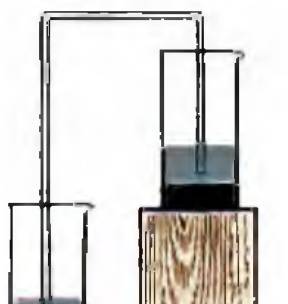
\includegraphics[width=0.86\linewidth]{rasmlar/darslik/d_tindirish.png}\end{center}
\noindent A)~\textsl{bug`latish}\par
\noindent B)~\textsl{dekantatsiya (tindirish)}\par
\noindent C)~\textsl{filtrlash}\par
\noindent D)~\textsl{distillash   ---}\par
\vspace{4pt}
\end{multicols}
\medskip
\noindent\setlength{\fboxsep}{0pt}\fbox{\begin{tabular}{p{0.74\linewidth}|p{0.2\linewidth}}
\parbox[t]{0.72\linewidth}{\vspace{3pt}\textbf{Topshiriqlar (33--35) va javob variant (A--F)larini o`zaro to`g`ri moslashtiring.} Propan (C\textsubscript{3}H\textsubscript{8}) va eten (C\textsubscript{2}H\textsubscript{4}) dan iborat 5,6 l (n.sh.) aralashma bromli suvdan o`tkazilganda 24 g brom yutildi.
\vspace{3pt}} & \parbox[t]{0.19\linewidth}{\vspace{3pt}A~\textsl{3,36}\\[3pt]
B~\textsl{30}\\[3pt]
C~\textsl{101,33}\\[3pt]
D~\textsl{202,67}\\[3pt]
E~\textsl{152}\\[3pt]
F~\textsl{60}}\\ \hline
\parbox[t]{0.72\linewidth}{\vspace{2pt}\textbf{33. Aralashmadagi eten (C\textsubscript{2}H\textsubscript{4}) hajmini (l, n.sh.) aniqlang.}\vspace{2pt}} & \\ \hline
\parbox[t]{0.72\linewidth}{\vspace{2pt}\textbf{34. Aralashmadagi eten (C\textsubscript{2}H\textsubscript{4}) hajmiy ulushini (\%) aniqlang.}\vspace{2pt}} & \\ \hline
\parbox[t]{0.72\linewidth}{\vspace{2pt}\textbf{35. Aralashmani to`liq yoqish uchun zarur havo hajmini (l, n.sh.; havoda 21\% kislorod bor) aniqlang.}\vspace{2pt}} & 
\end{tabular}}
\par\bigskip
\noindent\textbf{36.} Fe + H\textsubscript{2}SO\textsubscript{4} $\to$ Fe\textsubscript{2}(SO\textsubscript{4})\textsubscript{3} + SO\textsubscript{2} + H\textsubscript{2}O reaksiya tenglamasini tenglang va barcha koeffitsiyentlar \textbf{yig`indisini aniqlang.}
\javob
\noindent\textbf{37.} H\textsubscript{2}SO\textsubscript{4} ning 0,025 mol/l li eritmasidan 0,6 l va Ba(OH)\textsubscript{2} ning 0,025 mol/l li eritmasidan 0,4 l aralashtirildi (umumiy hajm 1 l, ikkala modda to`liq dissotsilanadi, BaSO\textsubscript{4} cho`kmasi e'tiborga olinmasin). Hosil bo`lgan eritmaning pH \textbf{ini aniqlang.}
\javob
\noindent\textbf{38.} NaBr va NaI dan iborat 17,8 g aralashma eritilib, mo`l xlor o`tkazildi, eritma bug`latilib quruq qoldiq 8,78 g chiqdi. Aralashmadagi NaI ning \textbf{massasini (g) toping.}
\javob
\noindent\textbf{39.} Etanol va fenoldan iborat 23,4 g aralashma natriy bilan to`liq reaksiyaga kirishganda 3,36 l (n.sh.) vodorod ajraldi. Shu aralashmaga mo`l bromli suv ta'sir ettirilganda hosil bo`ladigan cho`kma \textbf{massasini (g) toping.}
\javob
\noindent\textbf{40.} Polimerlanish darajasi 500 bo`lgan polipropilen ning 42 g namunasini olish uchun polimerlanish unumi 90\% bo`lganda qancha monomer (C\textsubscript{3}H\textsubscript{6}) kerak (g)?
\javob
\par\bigskip\begin{center}\textbf{\fontsize{13}{15}\selectfont YOZMA ISH}\end{center}
\noindent\textbf{41.} \textbf{Topshiriqni bajarish jarayonida barcha reaksiya tenglamalarini yozing. Miqdoriy va arifmetik hisoblashlarni (unga asos bo`lgan usul yoki formulani ko`rsatgan holda) uzviy ketma-ketlikda bajaring.}\par\smallskip
9,75 g noma'lum metall kislota bilan to`liq reaksiyaga kirishib, 3,36 l (n.sh.) vodorod ajratdi. (Vodorodning ekvivalent hajmi \textit{V}\_E(H\textsubscript{2}) = 11,2 l/mol.)\par
\noindent 1)Metallning ekvivalent massasini (g/mol) hisoblang.\par
\noindent 2)Metallning valentligi 2 bo`lsa, uning atom massasini hisoblab, metallni aniqlang. Ajralgan vodorodning massasini (g) ham hisoblang.\par
\noindent 3)Shu metallning oksidi formulasini yozing va molyar massasini hisoblang.\par
\noindent 4)9,75 g metall to`liq yonganda hosil bo`lgan oksid massasini (g) toping. Metall oksidining ekvivalent massasini (g/mol) ham aniqlang.\par
\noindent 5)Yonishga sarflangan kislorod hajmini (l, n.sh.) aniqlang. Shuningdek metall xloridida (MCl\textsubscript{2}) metallning massa ulushini (\%) toping.\par
\diqqat{Mazkur topshiriq kengaytirilgan javobni talab etib, uning yechilish usuli va shu usul asosidagi barcha hisoblash amallari javoblar varaqasida aks etishi lozim.}
\noindent\textbf{42.} Quyidagi o`zgarishlar zanjirida \textit{X}, \textit{Y}, \textit{Z} noma'lum organik moddalar:\par
\[\setlength{\fboxsep}{0pt}\text{CH\textsubscript{4}}\xrightarrow{\text{Cl\textsubscript{2}, yorug`lik}}\text{\textit{X}}\xrightarrow{\text{Na}}\text{\textit{Y}}\xrightarrow{\text{Cl\textsubscript{2}, yorug`lik}}\text{C\textsubscript{2}H\textsubscript{5}Cl}\]
\noindent 1)CH\textsubscript{4} $\to$ \textit{X} : reaksiya tenglamasini yozing; hosil bo`lgan moddani nomlang.\par
\noindent 2)\textit{X} $\to$ \textit{Y} : reaksiya tenglamasini yozing; hosil bo`lgan moddani nomlang.\par
\noindent 3)\textit{Y} $\to$ C\textsubscript{2}H\textsubscript{5}Cl : reaksiya tenglamasini yozing; hosil bo`lgan moddani nomlang.\par
\diqqat{Mazkur topshiriq kengaytirilgan javobni talab etib, uning yechilish usuli va shu usul asosidagi barcha hisoblash amallari javoblar varaqasida aks etishi lozim.}
\noindent\textbf{43.} \textbf{Topshiriqni bajarish jarayonida barcha reaksiya tenglamalarini yozing. Miqdoriy va arifmetik hisoblashlarni (unga asos bo`lgan usul yoki formulani ko`rsatgan holda) uzviy ketma-ketlikda bajaring.}\par\smallskip
50 m\textsuperscript{3} qattiq suvda Ca(HCO\textsubscript{3})\textsubscript{2} ning konsentratsiyasi 20 mol/m\textsuperscript{3}, Mg(HCO\textsubscript{3})\textsubscript{2} niki 10 mol/m\textsuperscript{3} ga teng (1 m\textsuperscript{3} = 1000 l).\par
\noindent 1)Suv qaynatilganda qanday reaksiyalar sodir bo`lishini yozing.\par
\noindent 2)Qaynatish natijasida hosil bo`ladigan CaCO\textsubscript{3} cho`kmasi massasini (kg) hisoblang. Qaynatish bilan ajralgan CO\textsubscript{2} hajmini (m\textsuperscript{3}, n.sh.) ham hisoblang.\par
\noindent 3)Mg(HCO\textsubscript{3})\textsubscript{2} dan hosil bo`ladigan MgCO\textsubscript{3} massasini (kg) toping.\par
\noindent 4)Suvni yumshatish uchun sodadan (Na\textsubscript{2}CO\textsubscript{3}) necha kilogramm kerakligini hisoblang (Ca\textsuperscript{2+} va Mg\textsuperscript{2+} ni to`liq cho`ktirish uchun).\par
\noindent 5)Suvni ohak sutini (Ca(OH)\textsubscript{2}) bilan yumshatishda zarur Ca(OH)\textsubscript{2} massasini (kg) hisoblang (Ca(HCO\textsubscript{3})\textsubscript{2} + Ca(OH)\textsubscript{2} $\to$ 2CaCO\textsubscript{3} + 2H\textsubscript{2}O; Mg(HCO\textsubscript{3})\textsubscript{2} + 2Ca(OH)\textsubscript{2} $\to$ Mg(OH)\textsubscript{2} + 2CaCO\textsubscript{3} + 2H\textsubscript{2}O).\par
\diqqat{Mazkur topshiriq kengaytirilgan javobni talab etib, uning yechilish usuli va shu usul asosidagi barcha hisoblash amallari javoblar varaqasida aks etishi lozim.}
\newpage
\noindent\textbf{\fontsize{13}{15}\selectfont Nazorat testi}\ \textit{$\cdot$ 9-variant}\hfill \textbf{Javoblar kaliti}\par\smallskip\hrule\smallskip
\textit{Faqat o`qituvchi uchun.}\par\medskip
\noindent\textbf{1--32-savollar}\par\smallskip
\noindent\begin{tabular}{|c|c|c|c|c|c|c|c|c|c|c|c|c|c|c|c|}\hline
\textbf{1} & \textbf{2} & \textbf{3} & \textbf{4} & \textbf{5} & \textbf{6} & \textbf{7} & \textbf{8} & \textbf{9} & \textbf{10} & \textbf{11} & \textbf{12} & \textbf{13} & \textbf{14} & \textbf{15} & \textbf{16}\\\hline
\textsl{A} & \textsl{B} & \textsl{B} & \textsl{D} & \textsl{A} & \textsl{B} & \textsl{B} & \textsl{C} & \textsl{D} & \textsl{C} & \textsl{A} & \textsl{D} & \textsl{C} & \textsl{C} & \textsl{D} & \textsl{A}\\\hline
\textbf{17} & \textbf{18} & \textbf{19} & \textbf{20} & \textbf{21} & \textbf{22} & \textbf{23} & \textbf{24} & \textbf{25} & \textbf{26} & \textbf{27} & \textbf{28} & \textbf{29} & \textbf{30} & \textbf{31} & \textbf{32}\\\hline
\textsl{A} & \textsl{C} & \textsl{B} & \textsl{C} & \textsl{B} & \textsl{C} & \textsl{D} & \textsl{D} & \textsl{A} & \textsl{D} & \textsl{A} & \textsl{D} & \textsl{C} & \textsl{A} & \textsl{B} & \textsl{B}\\\hline
\end{tabular}\par\medskip
\noindent\textbf{33--35-savollar}\par\smallskip
\noindent\begin{tabular}{|c|c|c|}\hline \textbf{No} & \textbf{Javob} & \textbf{Qiymat}\\\hline
33 & \textsl{A} & 3,36\\\hline
34 & \textsl{F} & 60\\\hline
35 & \textsl{C} & 101,33\\\hline
\end{tabular}\par\medskip
\noindent\textbf{36--40-savollar}\par\smallskip
\noindent\begin{tabular}{|c|c|}\hline \textbf{No} & \textbf{To`g`ri javob}\\\hline
36 & 18\\\hline
37 & 2\\\hline
38 & 7,5\\\hline
39 & 66,2\\\hline
40 & 46,67\\\hline
\end{tabular}\par\medskip
\noindent\textbf{41--43-topshiriqlar: qisqa yechim}\par\smallskip
\noindent\textbf{41-topshiriq.}\par
\noindent 1) E = m$\cdot$11,2/\textit{V} = 9,75$\cdot$11,2/3,36 = \textbf{32,5 g/mol}\par
\noindent 2) Ar = E$\cdot$valentlik = 32,5$\cdot$2 = 65 $\to$ \textbf{Zn}; m(H\textsubscript{2}) = 3,36/11,2 = \textbf{0,3 g}\par
\noindent 3) \textbf{ZnO}, M = \textbf{81 g/mol}\par
\noindent 4) m(oksid) = m + m(O) = 9,75 + 9,75$\cdot$8/32,5 = \textbf{12,15 g}; E(oksid) = E(Me) + 8 = \textbf{40,5 g/mol}\par
\noindent 5) m(O) = 2,4 g = 0,15 mol O $\to$ n(O\textsubscript{2}) = 0,075 mol $\to$ \textbf{1,68 l}; $\omega$ = 65/(65 + 71) = \textbf{47,8\%}\par
\noindent Jami: M 15 + A 10 = 25 ball.\par
\noindent\textbf{42-topshiriq.}\par
\noindent 1) CH\textsubscript{4} + Cl\textsubscript{2}, yorug`lik $\to$ CH\textsubscript{3}Cl (xlormetan)\par
\noindent 2) CH\textsubscript{3}Cl + Na $\to$ C\textsubscript{2}H\textsubscript{6} (etan)\par
\noindent 3) C\textsubscript{2}H\textsubscript{6} + Cl\textsubscript{2}, yorug`lik $\to$ C\textsubscript{2}H\textsubscript{5}Cl (xloretan)\par
\noindent Jami 25 ball.\par
\noindent\textbf{43-topshiriq.}\par
\noindent 1) Ca(HCO\textsubscript{3})\textsubscript{2} $\to$ CaCO\textsubscript{3}$\downarrow$ + CO\textsubscript{2}$\uparrow$ + H\textsubscript{2}O; Mg(HCO\textsubscript{3})\textsubscript{2} $\to$ MgCO\textsubscript{3}$\downarrow$ + CO\textsubscript{2}$\uparrow$ + H\textsubscript{2}O\par
\noindent 2) n(Ca(HCO\textsubscript{3})\textsubscript{2}) = 1000 mol $\to$ m(CaCO\textsubscript{3}) = \textbf{100 kg}; n(CO\textsubscript{2}) = n(Ca(HCO\textsubscript{3})\textsubscript{2}) + n(Mg(HCO\textsubscript{3})\textsubscript{2}) = 1500 mol $\to$ \textbf{33,6 m\textsuperscript{3}}\par
\noindent 3) n(Mg(HCO\textsubscript{3})\textsubscript{2}) = 500 mol $\to$ m(MgCO\textsubscript{3}) = \textbf{42 kg}\par
\noindent 4) Ca\textsuperscript{2+} + CO\textsubscript{3}\textsuperscript{2$-$} $\to$ CaCO\textsubscript{3}; Mg\textsuperscript{2+} + CO\textsubscript{3}\textsuperscript{2$-$} $\to$ MgCO\textsubscript{3}: n(Na\textsubscript{2}CO\textsubscript{3}) = 1500 mol $\to$ \textbf{159 kg}\par
\noindent 5) n(Ca(OH)\textsubscript{2}) = 1000 + 2$\cdot$500 = 2000 mol $\to$ \textbf{148 kg}\par
\noindent Jami: M 15 + A 10 = 25 ball.\par
\par\bigskip\noindent\textbf{Mavzular taqsimoti}\par\smallskip
{\small\noindent\begin{longtable}{|c|p{7.2cm}|p{5.4cm}|c|}\hline \textbf{No} & \textbf{Mavzu} & \textbf{Tekshiriladigan ko`nikma} & \textbf{Ball}\\\hline
1 & Tirkashev VI bob (reaksiya tezligi, grafik) & Grafik tahlili & 1\\\hline
2 & Tirkashev I bob; 8-sinf (izoelektron) & Bilim va tushunish & 1\\\hline
3 & Tirkashev III bob (eruvchanlik, jadval) & Jadval tahlili & 1\\\hline
4 & 9-sinf (gidroliz); Tirkashev IV bob & Bilim va tushunish & 1\\\hline
5 & Tirkashev VI bob (tezlik, jadval) & Jadval tahlili & 1\\\hline
6 & 8-sinf (kristall panjaralar) & Rasm bo`yicha tahlil & 1\\\hline
7 & 11-sinf 4-bob (normal konsentratsiya) & Hisoblash va masala yechish & 1\\\hline
8 & 11-sinf 8-bob (Faradey qonunlari); Tirkashev \textit{V} bob & Hisoblash va masala yechish & 1\\\hline
9 & Tirkashev VI bob & Hisoblash va masala yechish & 1\\\hline
10 & Tirkashev \textit{V} bob; 11-sinf 7-bob & Bilim va tushunish & 1\\\hline
11 & 11-sinf 8-bob; Tirkashev \textit{V} bob (elektroliz) & Bilim va tushunish & 1\\\hline
12 & 7-sinf (mol) & Hisoblash va masala yechish & 1\\\hline
13 & 11-sinf 4-bob (molyal konsentratsiya) & Hisoblash va masala yechish & 1\\\hline
14 & 9-sinf; Tirkashev (d-metallar (Fe,Cu,Zn,Cr), hisob) & Hisoblash va masala yechish & 1\\\hline
15 & 9-sinf; Tirkashev (suv qattiqligi, hisob) & Hisoblash va masala yechish & 1\\\hline
16 & 9-sinf; Tirkashev (oksid/asos/kislota/tuz, hisob) & Hisoblash va masala yechish & 1\\\hline
17 & 8-sinf; 9-sinf (genetik bog`lanish) & Bilim va tushunish & 1\\\hline
18 & 9-sinf; Tirkashev (mineral o`g`itlar/nodir gazlar, hisob) & Hisoblash va masala yechish & 1\\\hline
19 & Tashev (nitratlar) & Bilim va tushunish & 1\\\hline
20 & 10-sinf (alkan, hisob) & Hisoblash va masala yechish & 1\\\hline
21 & 10-sinf (mavzuga oid paragraflar); Abdusamatov & Bilim va tushunish & 1\\\hline
22 & 10-sinf (aren, hisob) & Hisoblash va masala yechish & 1\\\hline
23 & 10-sinf (mavzuga oid paragraflar); Abdusamatov & Bilim va tushunish & 1\\\hline
24 & 10-sinf \S{}24; \S{}26; \S{}30 (kumush ko`zgu) & Hisoblash va masala yechish & 1\\\hline
25 & 10-sinf (mavzuga oid paragraflar); Abdusamatov & Bilim va tushunish & 1\\\hline
26 & 10-sinf (mavzuga oid paragraflar); Abdusamatov & Bilim va tushunish & 1\\\hline
27 & 10-sinf (mavzuga oid paragraflar); Abdusamatov & Bilim va tushunish & 1\\\hline
28 & 10-sinf (amin, hisob) & Hisoblash va masala yechish & 1\\\hline
29 & 10-sinf \S{}35 (YuMB) & Hisoblash va masala yechish & 1\\\hline
30 & 7-sinf (aralashmalarni ajratish usullari) & Bilim va tushunish & 1\\\hline
31 & 9-sinf (sifat reaksiyalar) & Bilim va tushunish & 1\\\hline
32 & 7-sinf (aralashmalarni ajratish, 9-rasm) & Rasm bo`yicha tahlil & 1\\\hline
33--35 & Aralash masala (moslashtirish) & Ko`p bosqichli hisob & 3\\\hline
36--40 & Qisqa javobli masalalar & Hisoblash & 5\\\hline
41--43 & Yozma ish & Usul va hisob (M, A) & 75\\\hline
\end{longtable}}
\end{document}
